\chapter{Лабораторная работа 1 \\
Статические характеристики и цепи смещения транзисторных усилителей}

Цель работы: научиться измерять и анализировать статические характеристики усилителей на биполярном и полевом транзисторах, научиться проектировать схемы смещения усилителей на биполярном и полевом транзисторах, получить навыки работы со средой моделирования Advanced Design System.

\section{Техническое задание}

Определить выходные статические характеристики биполярного (HBFP0420) и полевого (MGF2148) транзисторов. Выбрать рабочую точку и расчитать цепь смещения.

\section{Выполнение работы}

\subsection{Измерение выходных статических характеристик биполярного транзистора}

Для измерения выходных статических характеристик биполярного транзистора необходимо собрать модель, показанную на рис.~\ref{fig:bias_circuits_bipolar_schematic_1}.

\begin{figure}
    \centering
    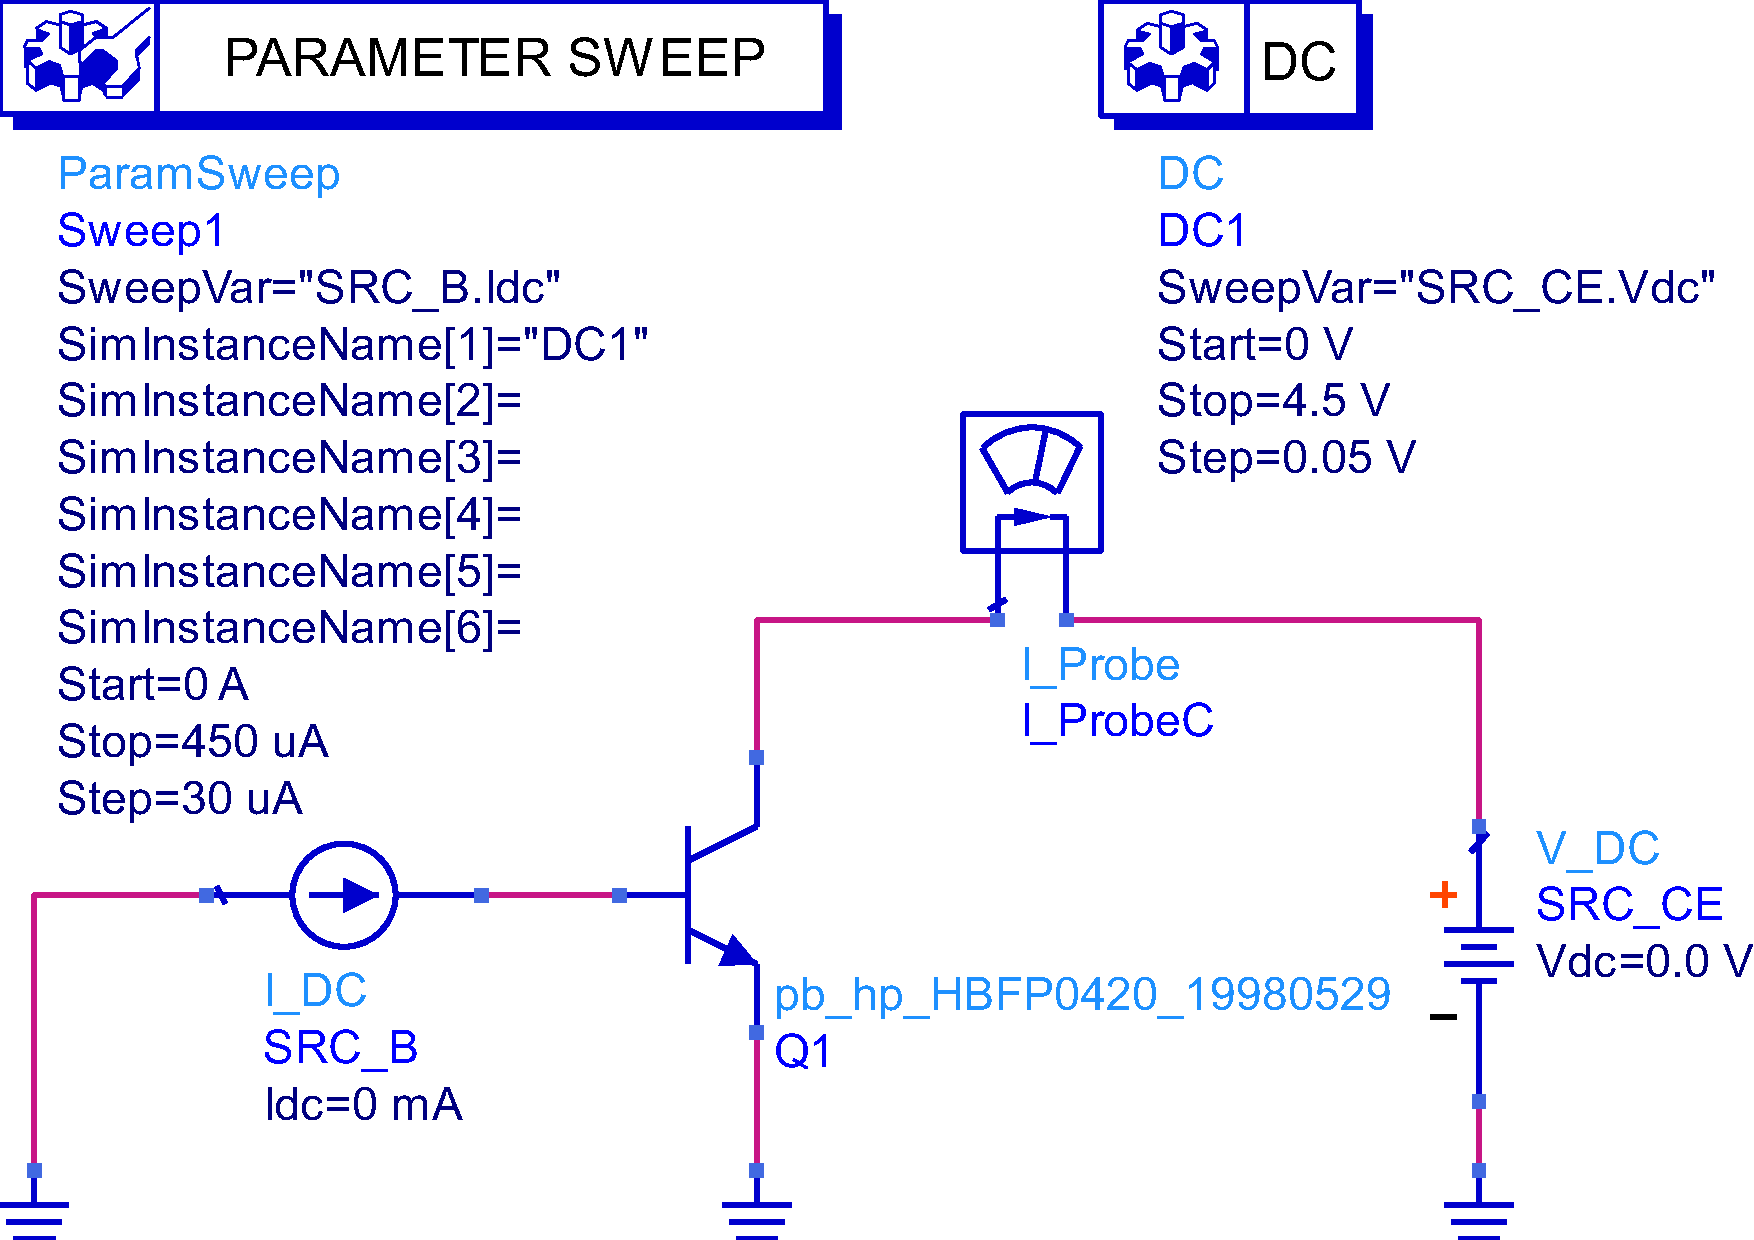
\includegraphics[width=0.8\textwidth]{bias_circuits_bipolar_schematic_1}
    \caption{Схема для измерения выходных статических характеристик биполярного транзистора}%
    \label{fig:bias_circuits_bipolar_schematic_1}
\end{figure}

Источник постоянного напряжения \elementname{SRC\_CE} задает напряжение коллектор-эмиттер и источник постоянного тока \elementname{SRC\_B} задает ток базы.
Ток коллектора измеряется с помощью \elementname{I\_ProbeC}.
В свойствах симулятора DC1 задается диапазон изменения напряжения коллектор-эмиттер (независимая переменная) и в дополнительном блоке \elementname{Ib\_Sweep} задается набор тока базы.
Предел напряжения коллектор-эмиттер брать от 0 В до предельно допустимого из рекомендаций производителя. Предел тока базы брать от 0 А до предельно допустимого из рекомендаций производителя.
Измеряемое семейство графиков будет выглядеть как показано на рис.~\ref{fig:bias_circuits_bipolar_data_display_1}.

\begin{figure}
    \centering
    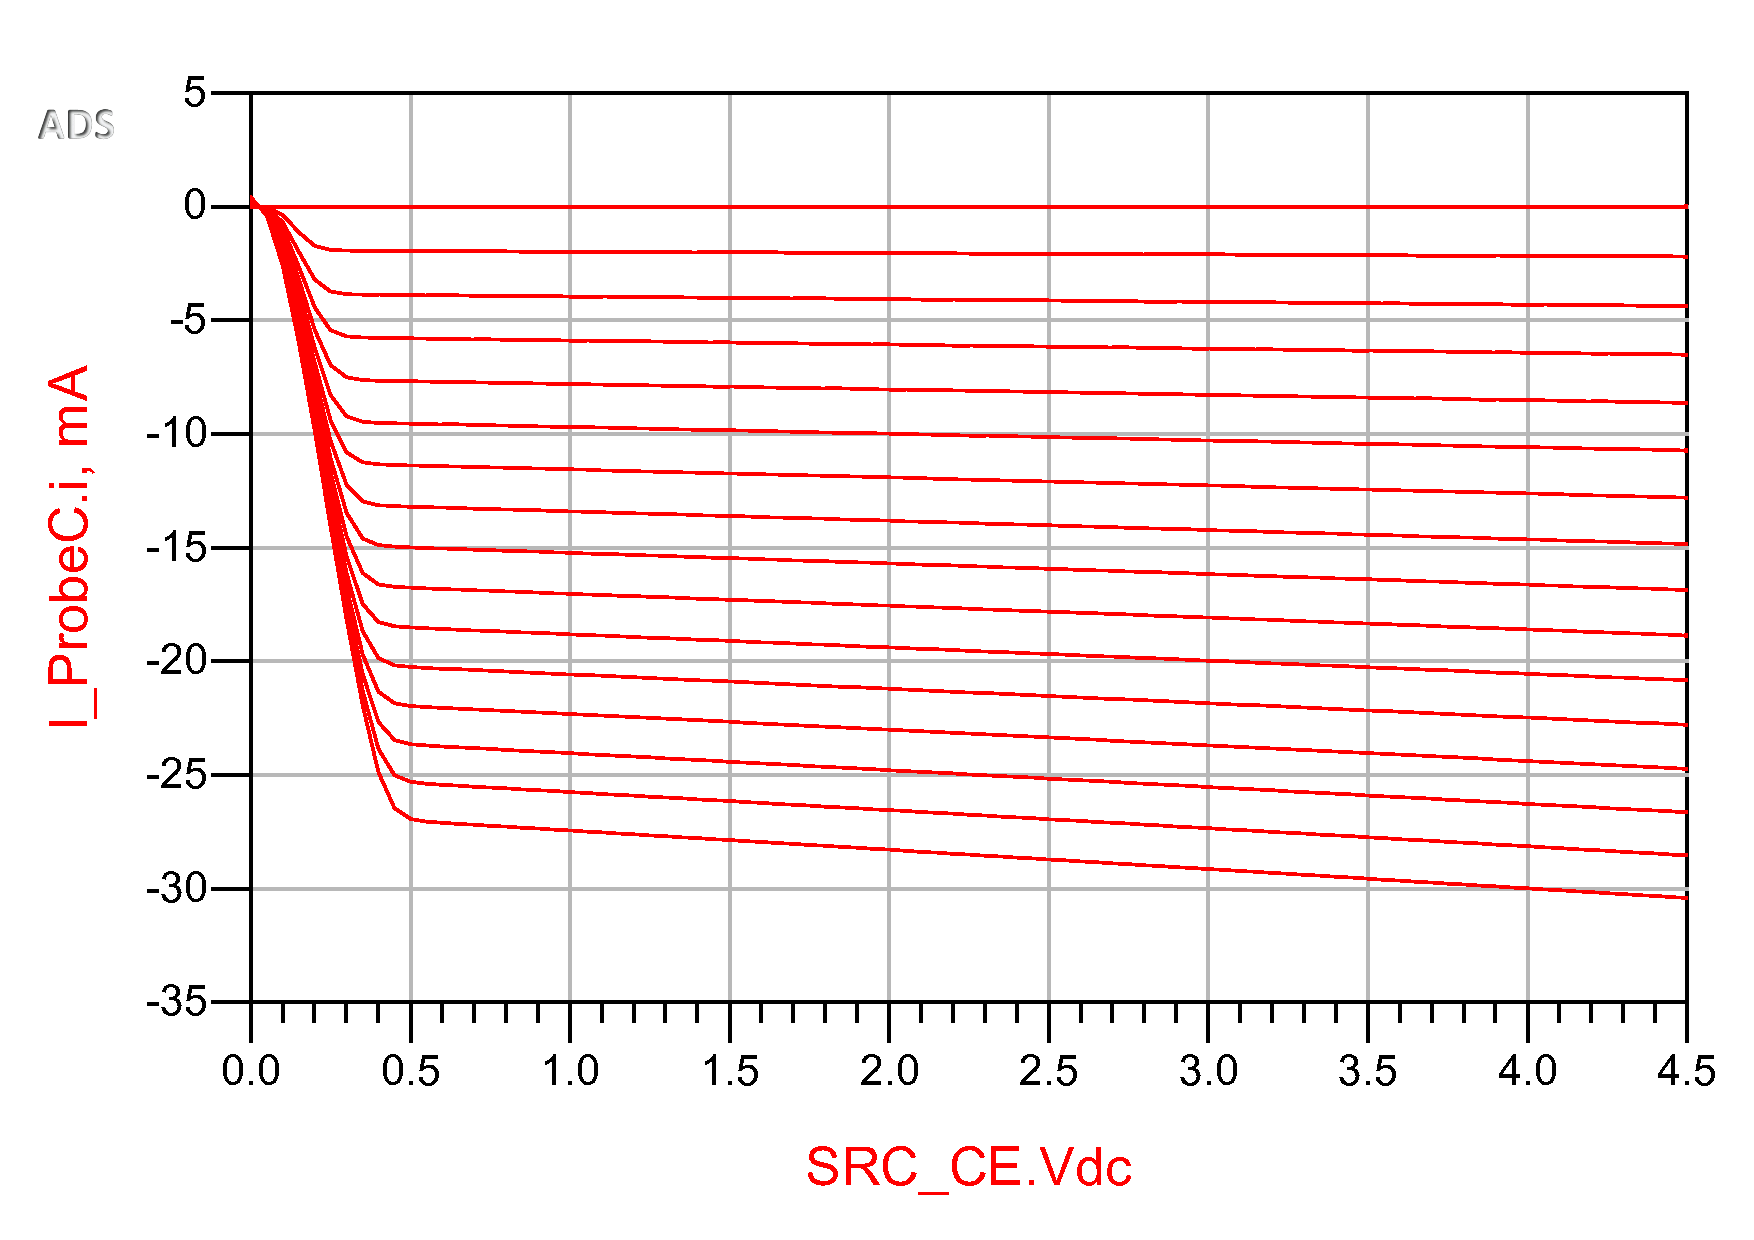
\includegraphics[width=0.8\textwidth]{bias_circuits_bipolar_data_display_1}
    \caption{Выходные статические характеристики биполярного транзистора}%
    \label{fig:bias_circuits_bipolar_data_display_1}
\end{figure}

\subsection{Измерение выходных статических характеристик полевого транзистора}

Для измерения выходных статических характеристик биполярного транзистора необходимо собрать модель, показанную на рис.~\ref{fig:bias_circuits_field_schematic}.

\begin{figure}
    \centering
    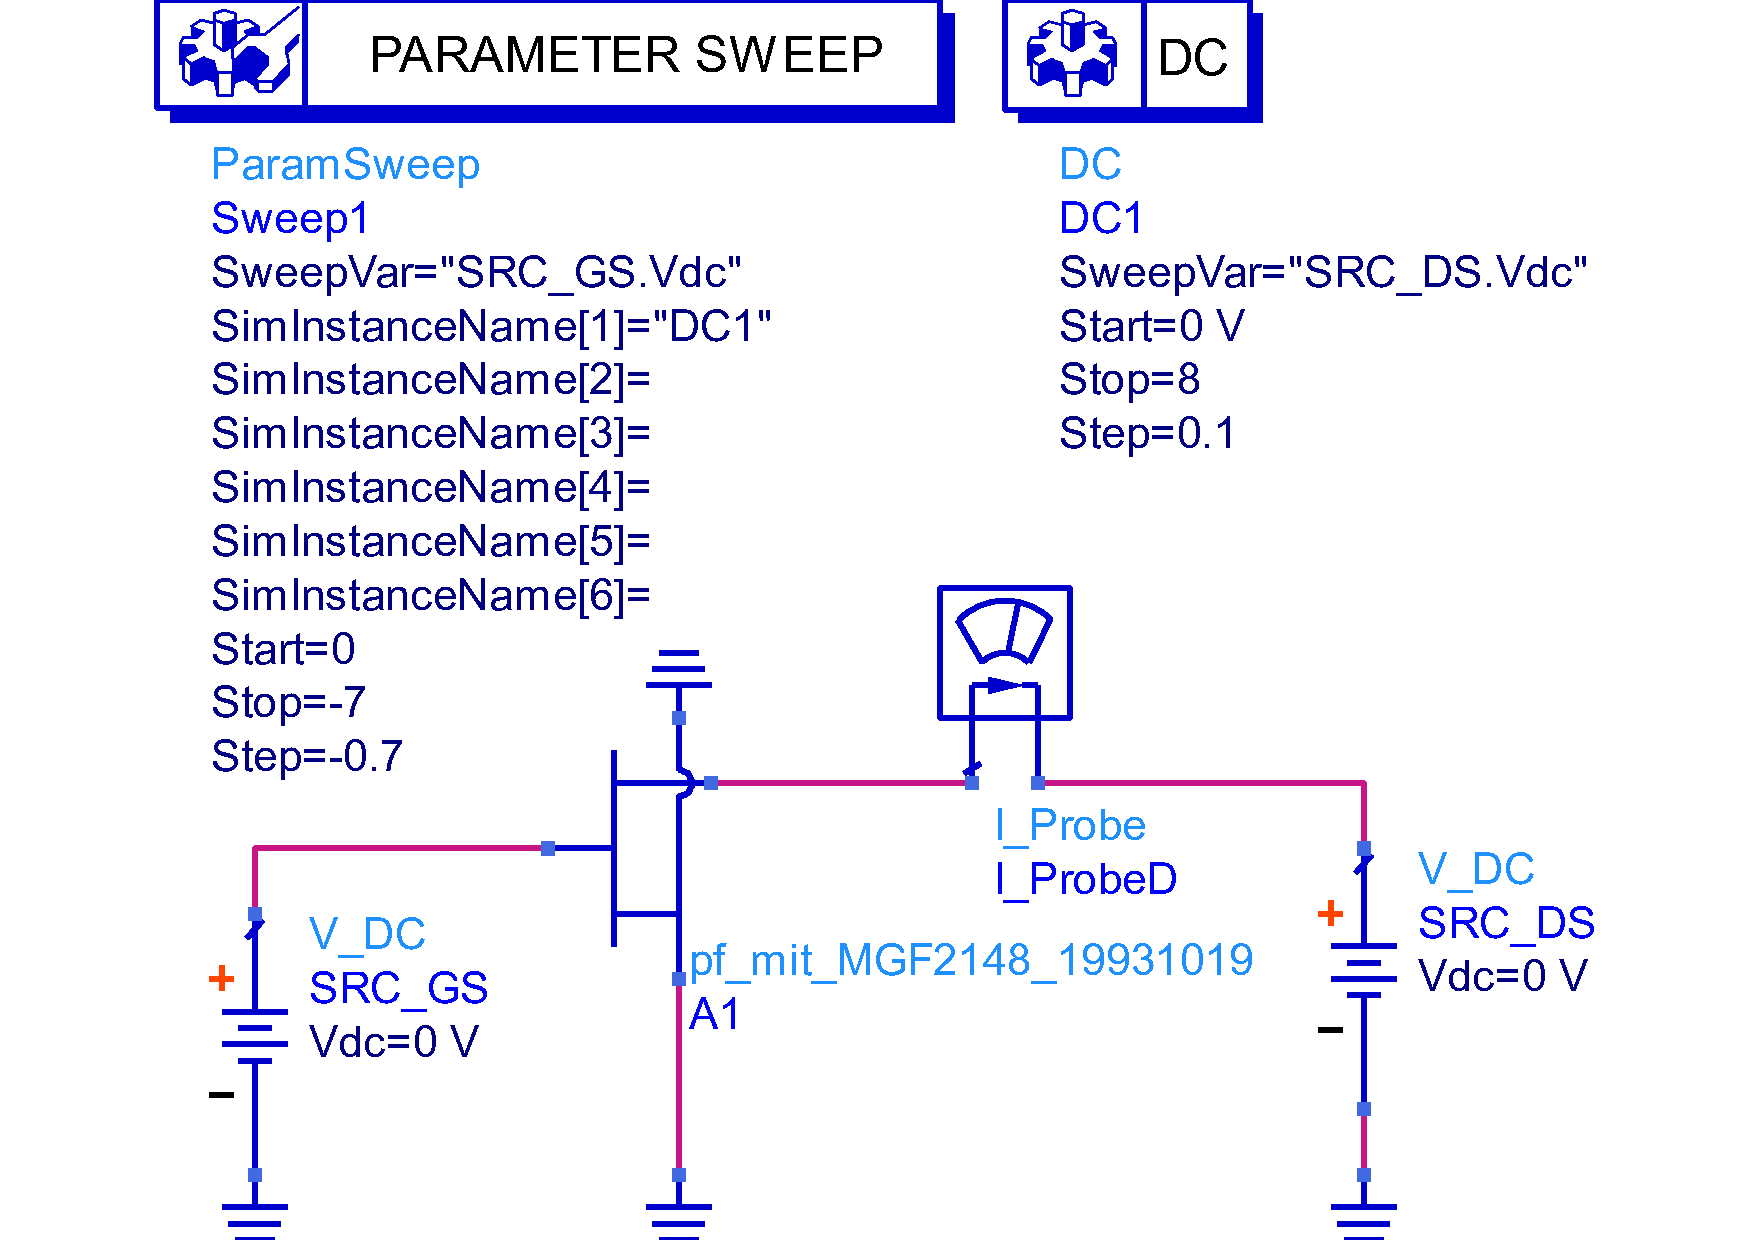
\includegraphics[width=0.8\textwidth]{bias_circuits_field_schematic}
    \caption{Схема для измерения выходных статических характеристик полевого транзистора}%
    \label{fig:bias_circuits_field_schematic}
\end{figure}

Два источника постоянного напряжения \elementname{SRC\_GS} и \elementname{SRC\_DS} задают напряжения затвор-исток (gate-source) и сток-исток (drain-source) соответственно.
Ток стока измеряется с помощью \elementname{I\_ProbeD}. В свойствах симулятора \elementname{DC1} задается диапазон изменения напряжения сток-исток (независимая переменная) и в дополнительном блоке \elementname{VGS\_Sweep} задается набор напряжений затвор-исток.

Предел напряжения сток-исток брать от 0~В до предельно допустимого из рекомендаций производителя. Предел напряжения затвор-исток тока базы брать от предельно допустимого из рекомендаций производителя до 0~В.

Измеряемое семейство графиков будет выглядеть как показано на рис.~\ref{fig:bias_circuits_field_data_display}.

\begin{figure}
    \centering
    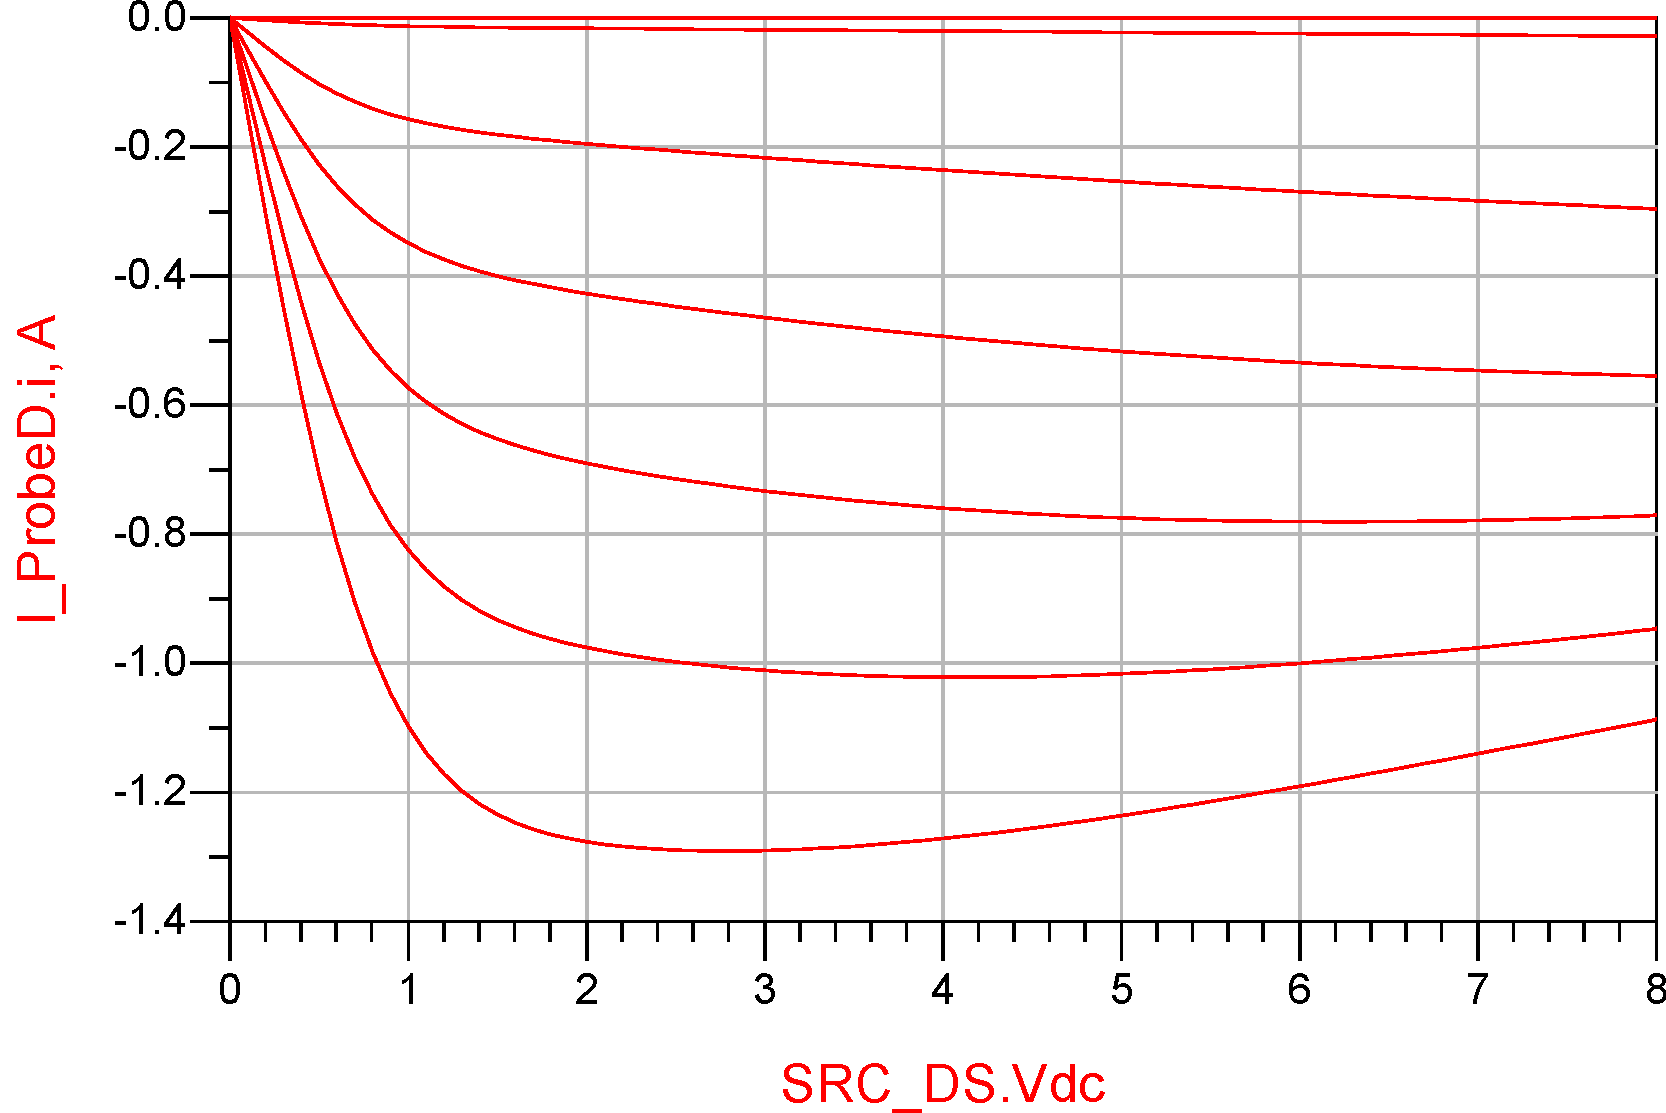
\includegraphics[width=0.8\textwidth]{bias_circuits_field_data_display}
    \caption{Выходные статические характеристики полевого транзистора}%
    \label{fig:bias_circuits_field_data_display}
\end{figure}
